\section{Introdução}

\begin{frame}
  \frametitle{\emph{Main Achievement} deste trabalho}

    Monitorar a posição de qualquer objeto no espaço usando RF-ID.

    \begin{itemize}
      \item Com \alert{alta precisão} (erro de 3.5 cm)
      \item Em \alert{tempo real}
      \item Funciona mesmo em ambientes \alert{indoor}
    \end{itemize}
\end{frame}

\section{E para que serve isso?}

\begin{frame}
  \begin{center}
    \Huge E para que serve isso?
  \end{center}
\end{frame}

\begin{frame}
  \frametitle{Interação homem-máquina}
  \begin{itemize}
    \item  Controle/monitoração de braços robóticos
  \end{itemize}

  \begin{center}
    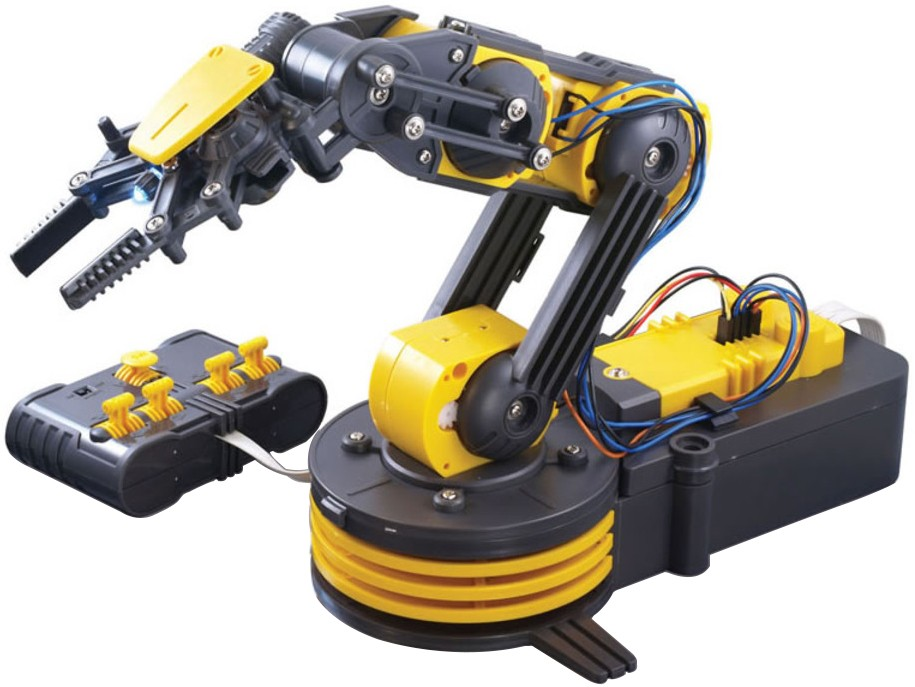
\includegraphics[width=.8\textwidth]{robot-arm}
  \end{center}
  %TODO
\end{frame}

\begin{frame}
  \frametitle{Interação homem-máquina}
  \begin{itemize}
    \item  Carros autônomos
  \end{itemize}

  \begin{center}
    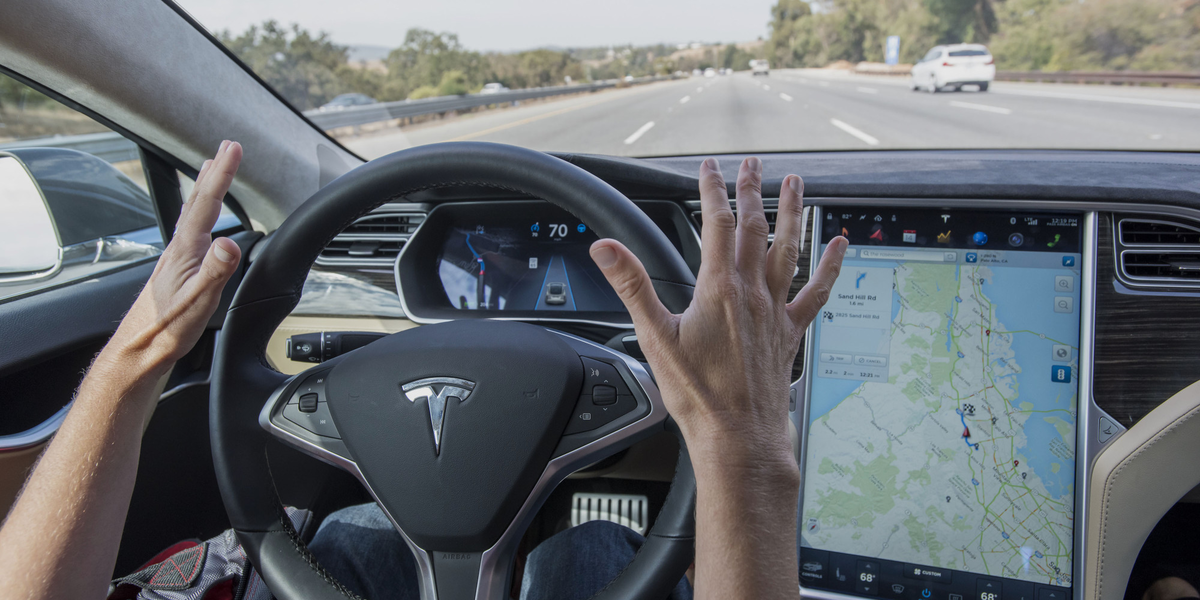
\includegraphics[width=\textwidth]{autopilot}
  \end{center}
\end{frame}

\begin{frame}
  \frametitle{Jogos / Realidade aumentada}
  \begin{itemize}
    \item  Kinect
    \item  Wii
  \end{itemize}
  %TODO
\end{frame}

\begin{frame}
  \frametitle{Aplicações comerciais}
  \begin{itemize}
    \item  Amazon store
    \item  Controle de estoque
  \end{itemize}
  %TODO
\end{frame}

\begin{frame}
  \frametitle{3D-Tracking hoje}

  Boa parte das técnicas de 3D-Tracking atuais são baseadas em visão computacional, com pequenas variações:
  \begin{itemize}
    \item no número de câmeras utilizadas
    \item nos algoritmos de CV utilizados
    \item etc
  \end{itemize}
\end{frame}

\begin{frame}
  \frametitle{O problema já não está então resolvido?}

  Limitações das soluções atuais
  \begin{itemize}
    \item  Alta complexidade computacional
    \item  Custo de implementação
    \item  Não funcionam em ambientes com obstáculos
  \end{itemize}

  %TODO: Adicionar figura
\end{frame}


\begin{frame}
  \frametitle{3D-Tracking com RF-ID}

  Vantagens
  \begin{itemize}
    \item  Tags são muito baratas ($0.1 \sim 0.2$ dólares)!
    \item  Técnica funciona mesmo com obstáculos
    \item  Menor complexidade computacional!
  \end{itemize}

  Problemas do estado-da-arte que a técnica que apresentaremos supera
  \begin{itemize}
    \item  Dependência de antenas de referência ou \emph{anchor nodes} 
    \item  Dependência de conhecimento prévio da trajetória
    \item  Limitação a 2D-Tracking
  \end{itemize}
\end{frame}
